%% ----------------------------------------------------------------
%% Authoring.tex
%% ---------------------------------------------------------------- 
\chapter{Authoring Tool} \label{Chapter:Authoring Tool}
An authoring tool was required to allow users to create their own question sets. This also avoids the necessity to use hardcoded files. The options given were based on the metadata that would be exported as a JSON file, as specified for the video overlay.

The authoring tool allows users to create polls and quizzes and overlay them at the desired locations in videos. The video chosen would come from a URL and question sets can be added at any point in the video. There could be any number of questions in a set and these could be of many different types.
\section{Design} \label{Section:Design}
As the rest of the project uses a bootstrap and Angular approach it was decided to use this for the authoring tool. This led to the use of UIBootstrap. Wireframes were created using this style so that they could easily be directly coded as static HTML to allow a quick demo to be created. 

Two different approaches were suggested for showing the advanced options for the video. A pop up approach hid these from general view to avoid confusing users with lots of options that may be unecessary. The other approach was to use the accordian structure as we had for the questions. This would be collapsed by default so the options would still be hidden. This was chosen as it was more consistent with the rest of the tool.

%Put wireframes in annex??
\begin{figure}[h]
	\centering 
	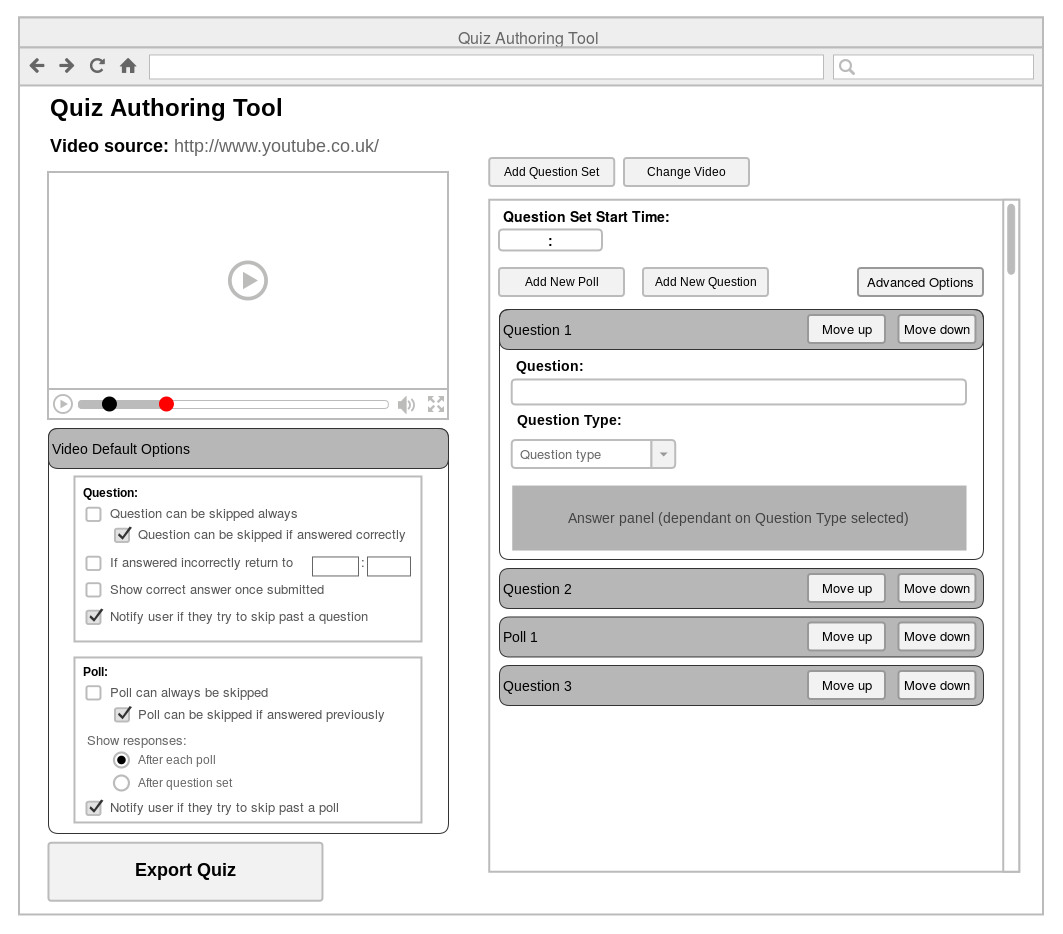
\includegraphics[scale=0.2]{../../authoring-tool/wireframes/gdpAuthoringAccordianVideoDefaultOptions.png} 	
	\caption{\label{fig:sift} Accordian approach wireframe } 	
\end{figure}